\documentclass[aspectratio=169,11pt]{beamer}

\usepackage[utf8]{inputenc}
\usepackage[spanish]{babel}
\usepackage{graphicx}
\usepackage{xcolor}

\graphicspath{{../latex/figures/}}

\definecolor{navy}{HTML}{103654}
\definecolor{teal}{HTML}{1C7C7D}
\definecolor{gold}{HTML}{D79B2E}
\definecolor{textgray}{HTML}{1F252B}

\setbeamercolor{structure}{fg=navy}
\setbeamercolor{title}{fg=navy}
\setbeamercolor{frametitle}{fg=navy,bg=white}
\setbeamercolor{normal text}{fg=textgray,bg=white}
\setbeamercolor{block title}{fg=white,bg=navy}
\setbeamercolor{block body}{fg=textgray,bg=white}
\setbeamertemplate{navigation symbols}{}

\title{Precisión estructural real de AlphaFold2 tras corregir el mapeo PDB--UniProt}
\subtitle{Benchmark con SIFTS en 10,432 proteínas únicas}
\author{José Antonio Tapia Godínez}
\institute{Maestría en Ciencia de Datos, ITAM}
\date{Concurso de Posters de Titulación 2026}

\begin{document}

\begin{frame}
  \titlepage
\end{frame}

\begin{frame}[t,shrink=8]{Problema y objetivo}
  \small
  \begin{block}{Problema}
    Las comparaciones PDB--AlphaFold2 sin mapeo posicional reportan RMSD mediano de \textbf{22.54 \AA} (solo 13.9\% bajo 2 \AA), sugiriendo fallo masivo del modelo. Esto contradice CASP14 (GDT 92.4/100, equivalente a variabilidad experimental). La discrepancia exige explicación.
  \end{block}

  \begin{block}{Objetivo}
    Determinar la precisión real de AlphaFold2 con un pipeline reproducible basado en:
    \begin{itemize}
      \item selección diversa por identificador UniProt,
      \item mapeo SIFTS a nivel residuo,
      \item superposición Kabsch y RMSD de C$\alpha$.
    \end{itemize}
  \end{block}

  \begin{block}{Datos}
    \begin{itemize}
      \item 13,000 pares candidatos PDB--AlphaFold2.
      \item 11,384 pares descargados con ambos archivos.
      \item \textbf{10,432 proteínas únicas} procesadas con SIFTS (91.6\%).
    \end{itemize}
  \end{block}
\end{frame}

\begin{frame}[t,shrink=8]{Diseño metodológico}
  \small
  \begin{columns}[T]
    \column{0.56\textwidth}
      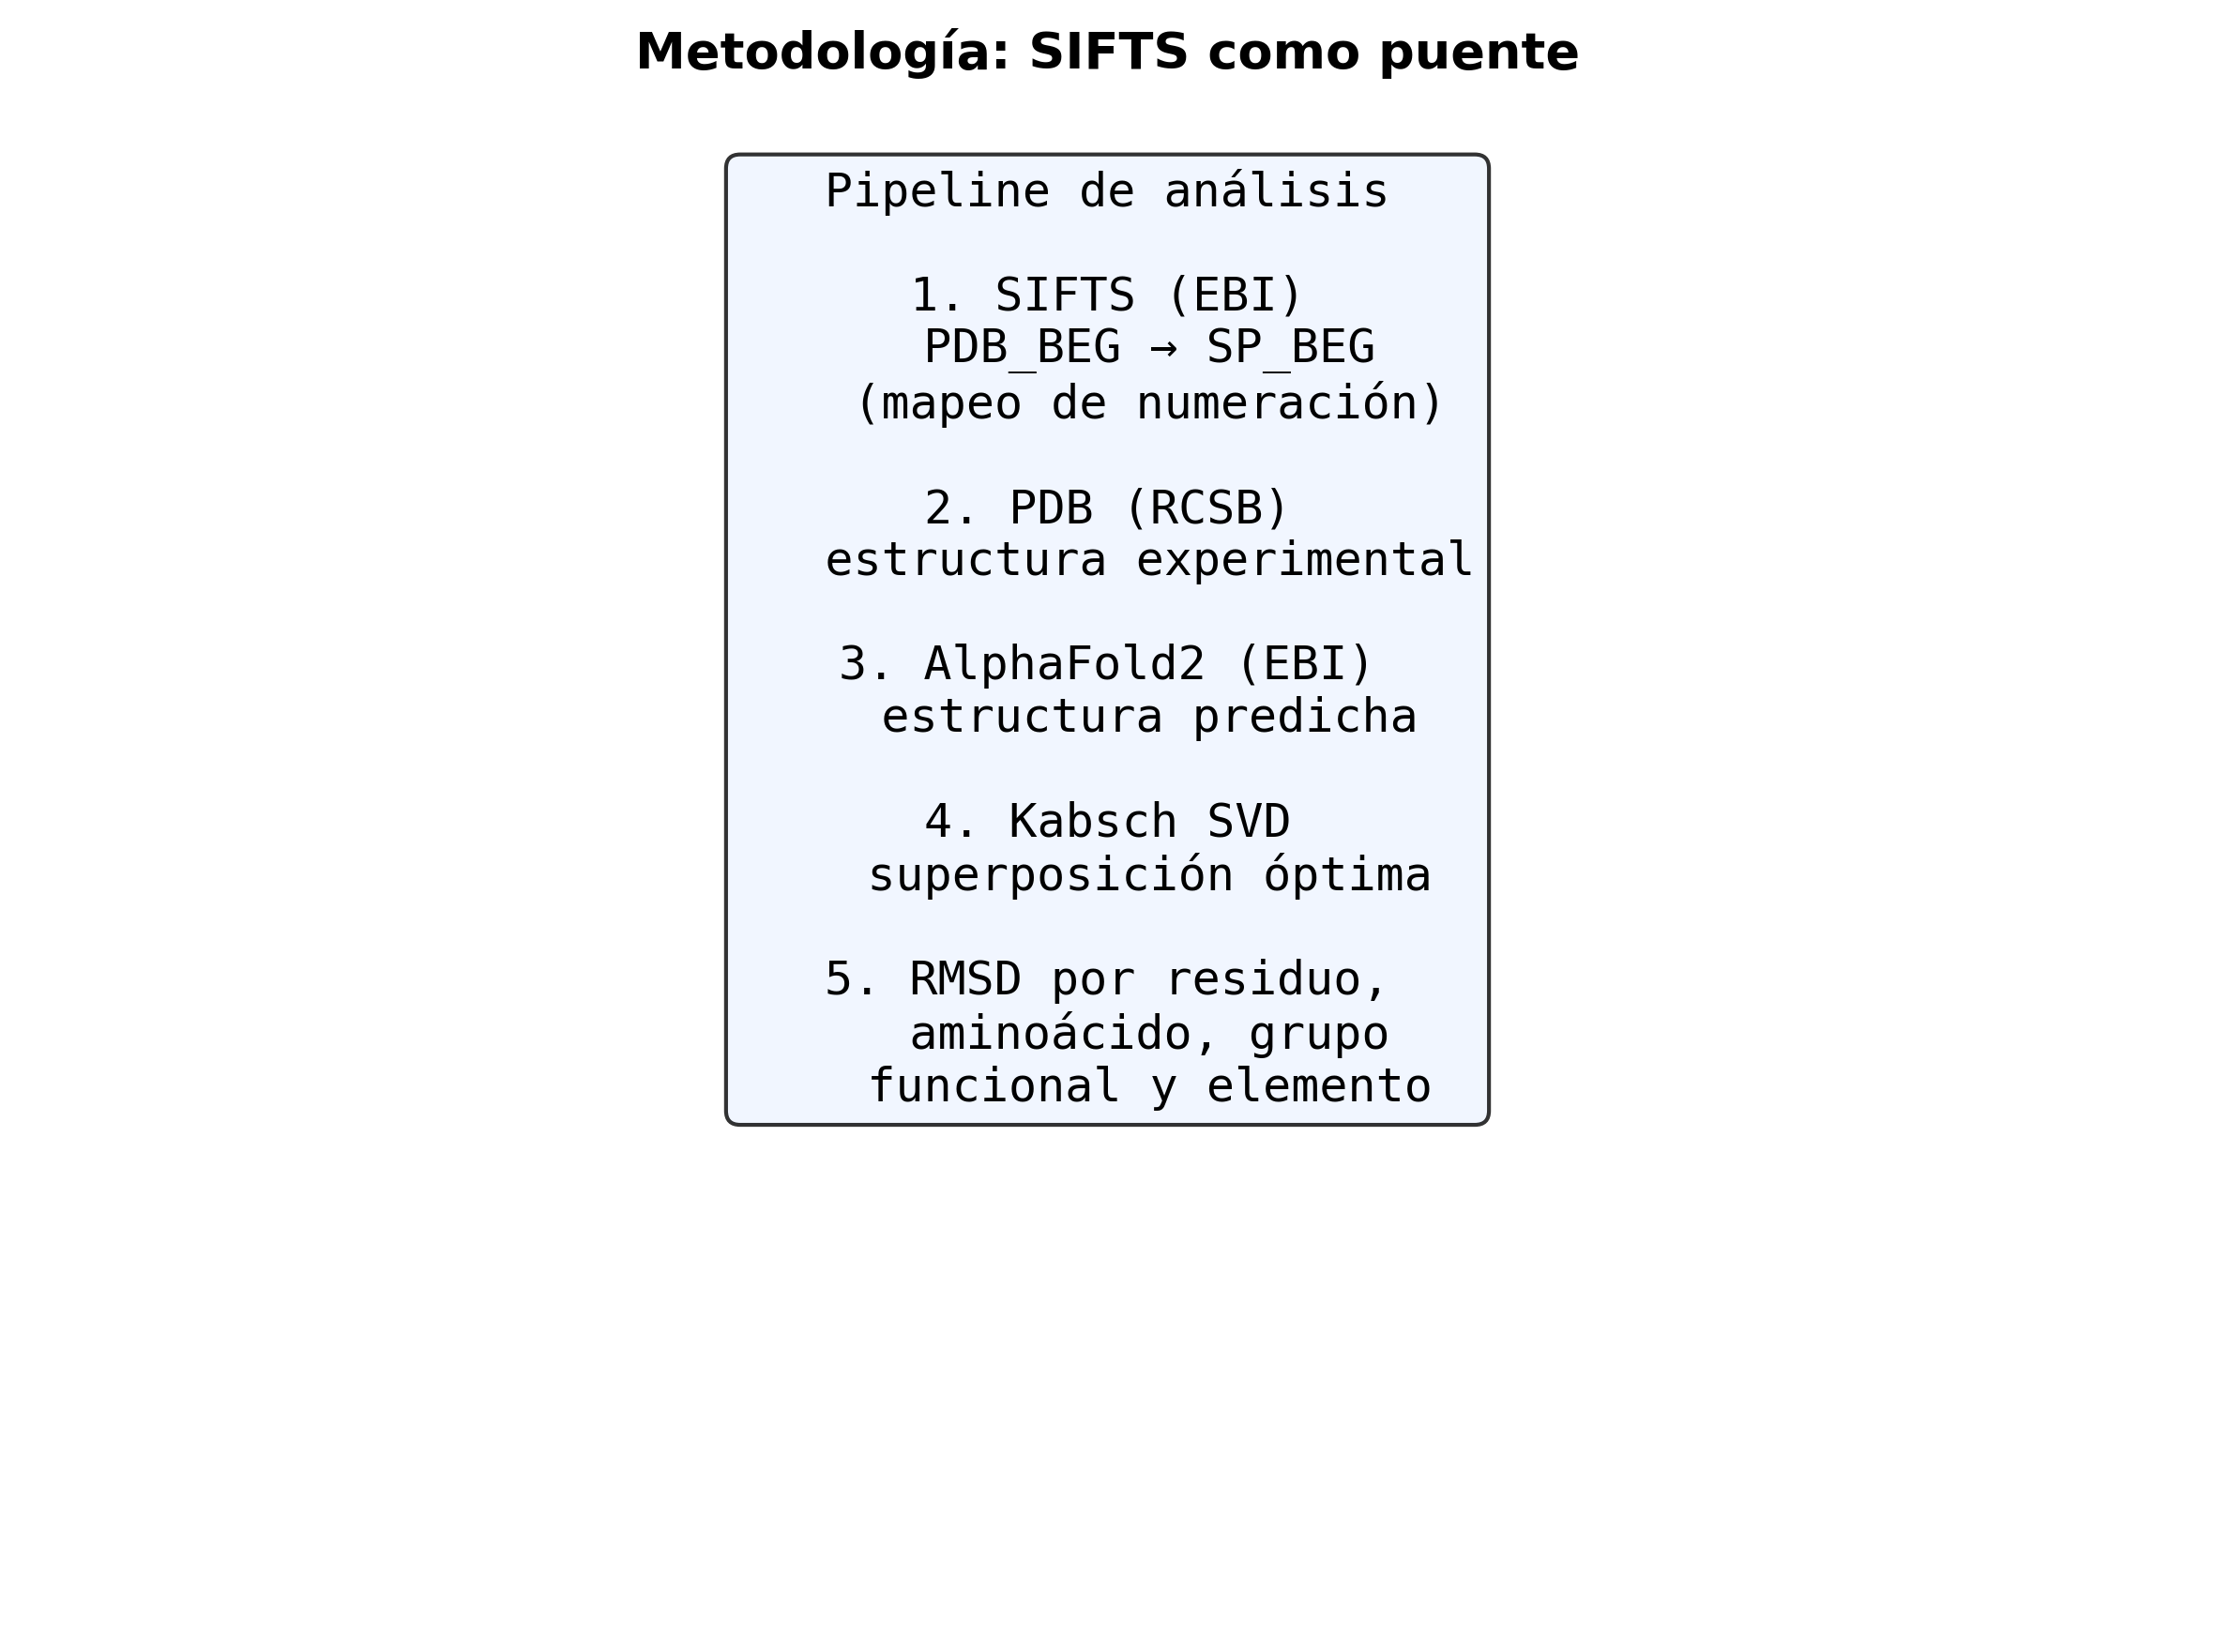
\includegraphics[width=0.97\linewidth]{fig_00a_pipeline.png}
    \column{0.42\textwidth}
      \begin{block}{Decisiones clave}
        \begin{itemize}
          \item \textbf{PDB} como referencia experimental ($>$200K estructuras).
          \item \textbf{AF2} (CASP14: GDT 92.4/100, AFDB: $>$200M proteínas).
          \item \textbf{SIFTS} corrige numeración y selección de cadena.
          \item \textbf{Kabsch} para superposición óptima.
        \end{itemize}
      \end{block}

      \begin{block}{Variables}
        \begin{itemize}
          \item \textbf{Respuesta:} RMSD de C$\alpha$ tras alineamiento.
          \item \textbf{Estructurales:} longitud, residuos mapeados.
          \item \textbf{Químicas:} aminoácido, grupo funcional, elemento.
        \end{itemize}
      \end{block}
  \end{columns}
\end{frame}

\begin{frame}{Hallazgo metodológico central}
  \begin{columns}[T]
    \column{0.60\textwidth}
      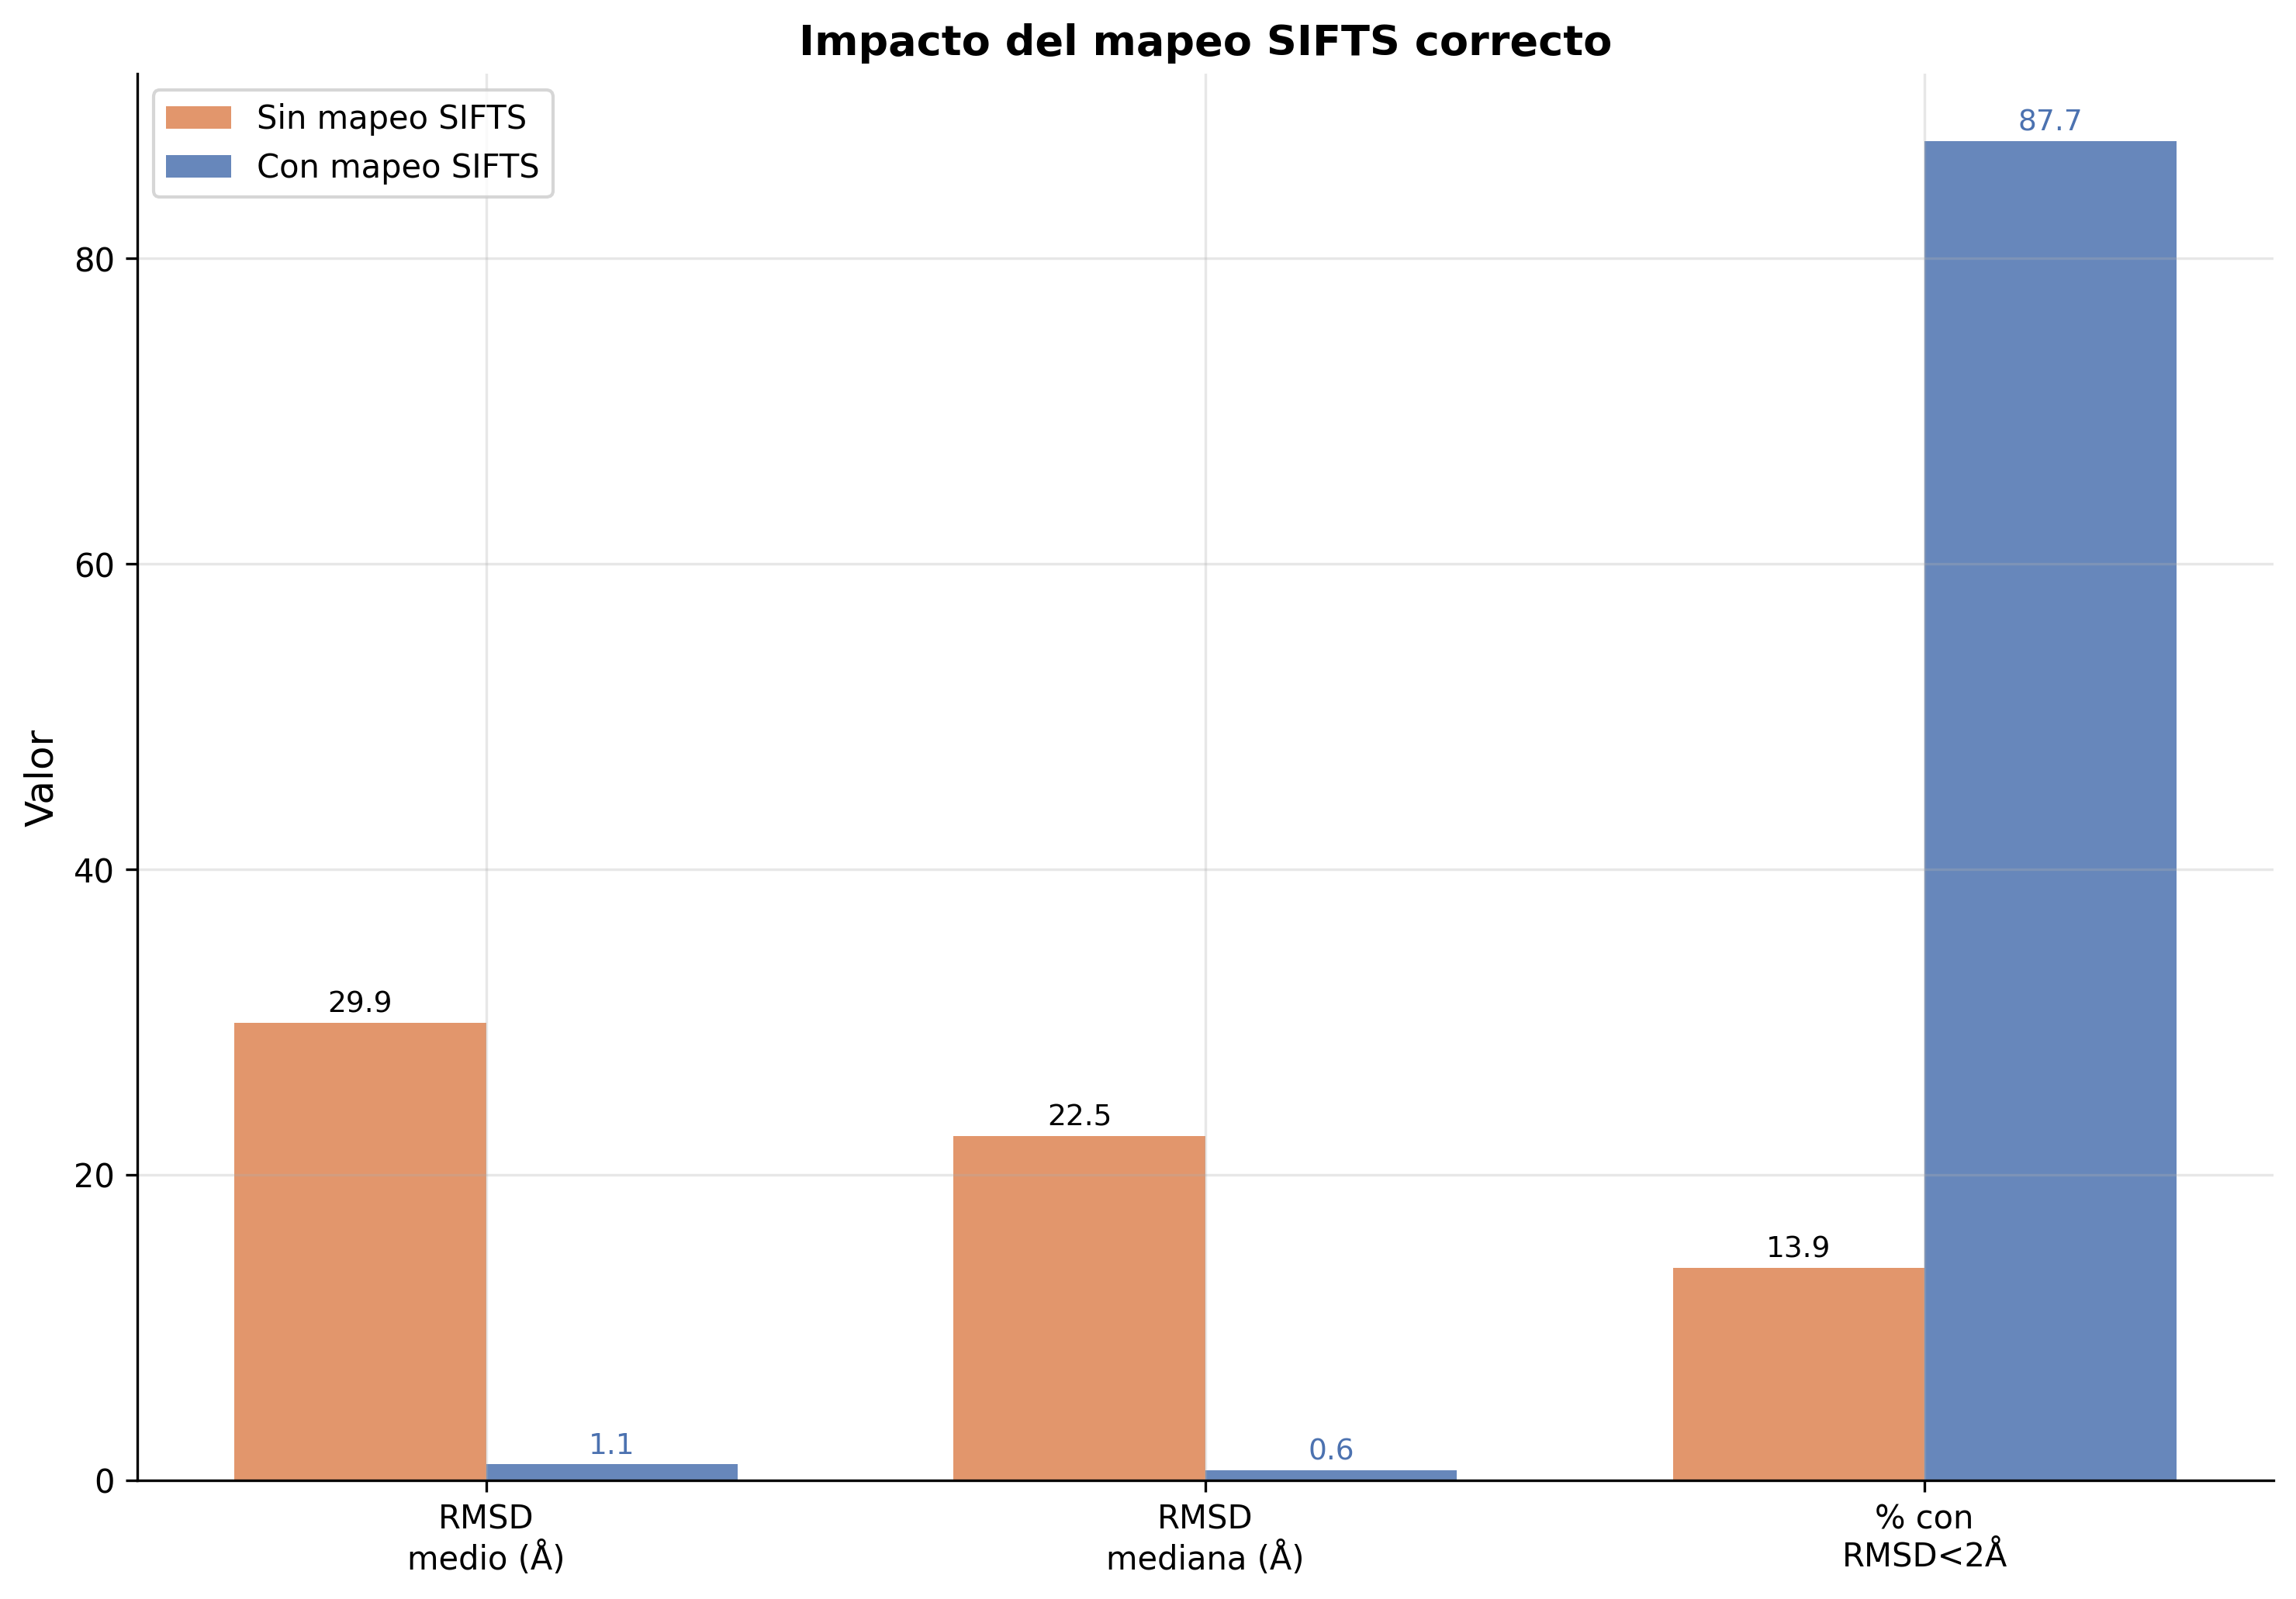
\includegraphics[width=\linewidth]{fig_00b_sifts_comparison.png}
    \column{0.37\textwidth}
      \begin{block}{Efecto de usar SIFTS}
        \begin{itemize}
          \item RMSD medio: 29.94 \AA{} $\rightarrow$ 1.05 \AA
          \item RMSD mediano: 22.54 \AA{} $\rightarrow$ 0.64 \AA
          \item RMSD $<2$ \AA: 13.9\% $\rightarrow$ 87.7\%
        \end{itemize}
      \end{block}

      \begin{alertblock}{Interpretación}
        La mayor parte del error previo provenía de un artefacto de alineación, no de un fallo masivo de AlphaFold2.
      \end{alertblock}
  \end{columns}
\end{frame}

\begin{frame}{Resultados globales}
  \begin{columns}[T]
    \column{0.58\textwidth}
      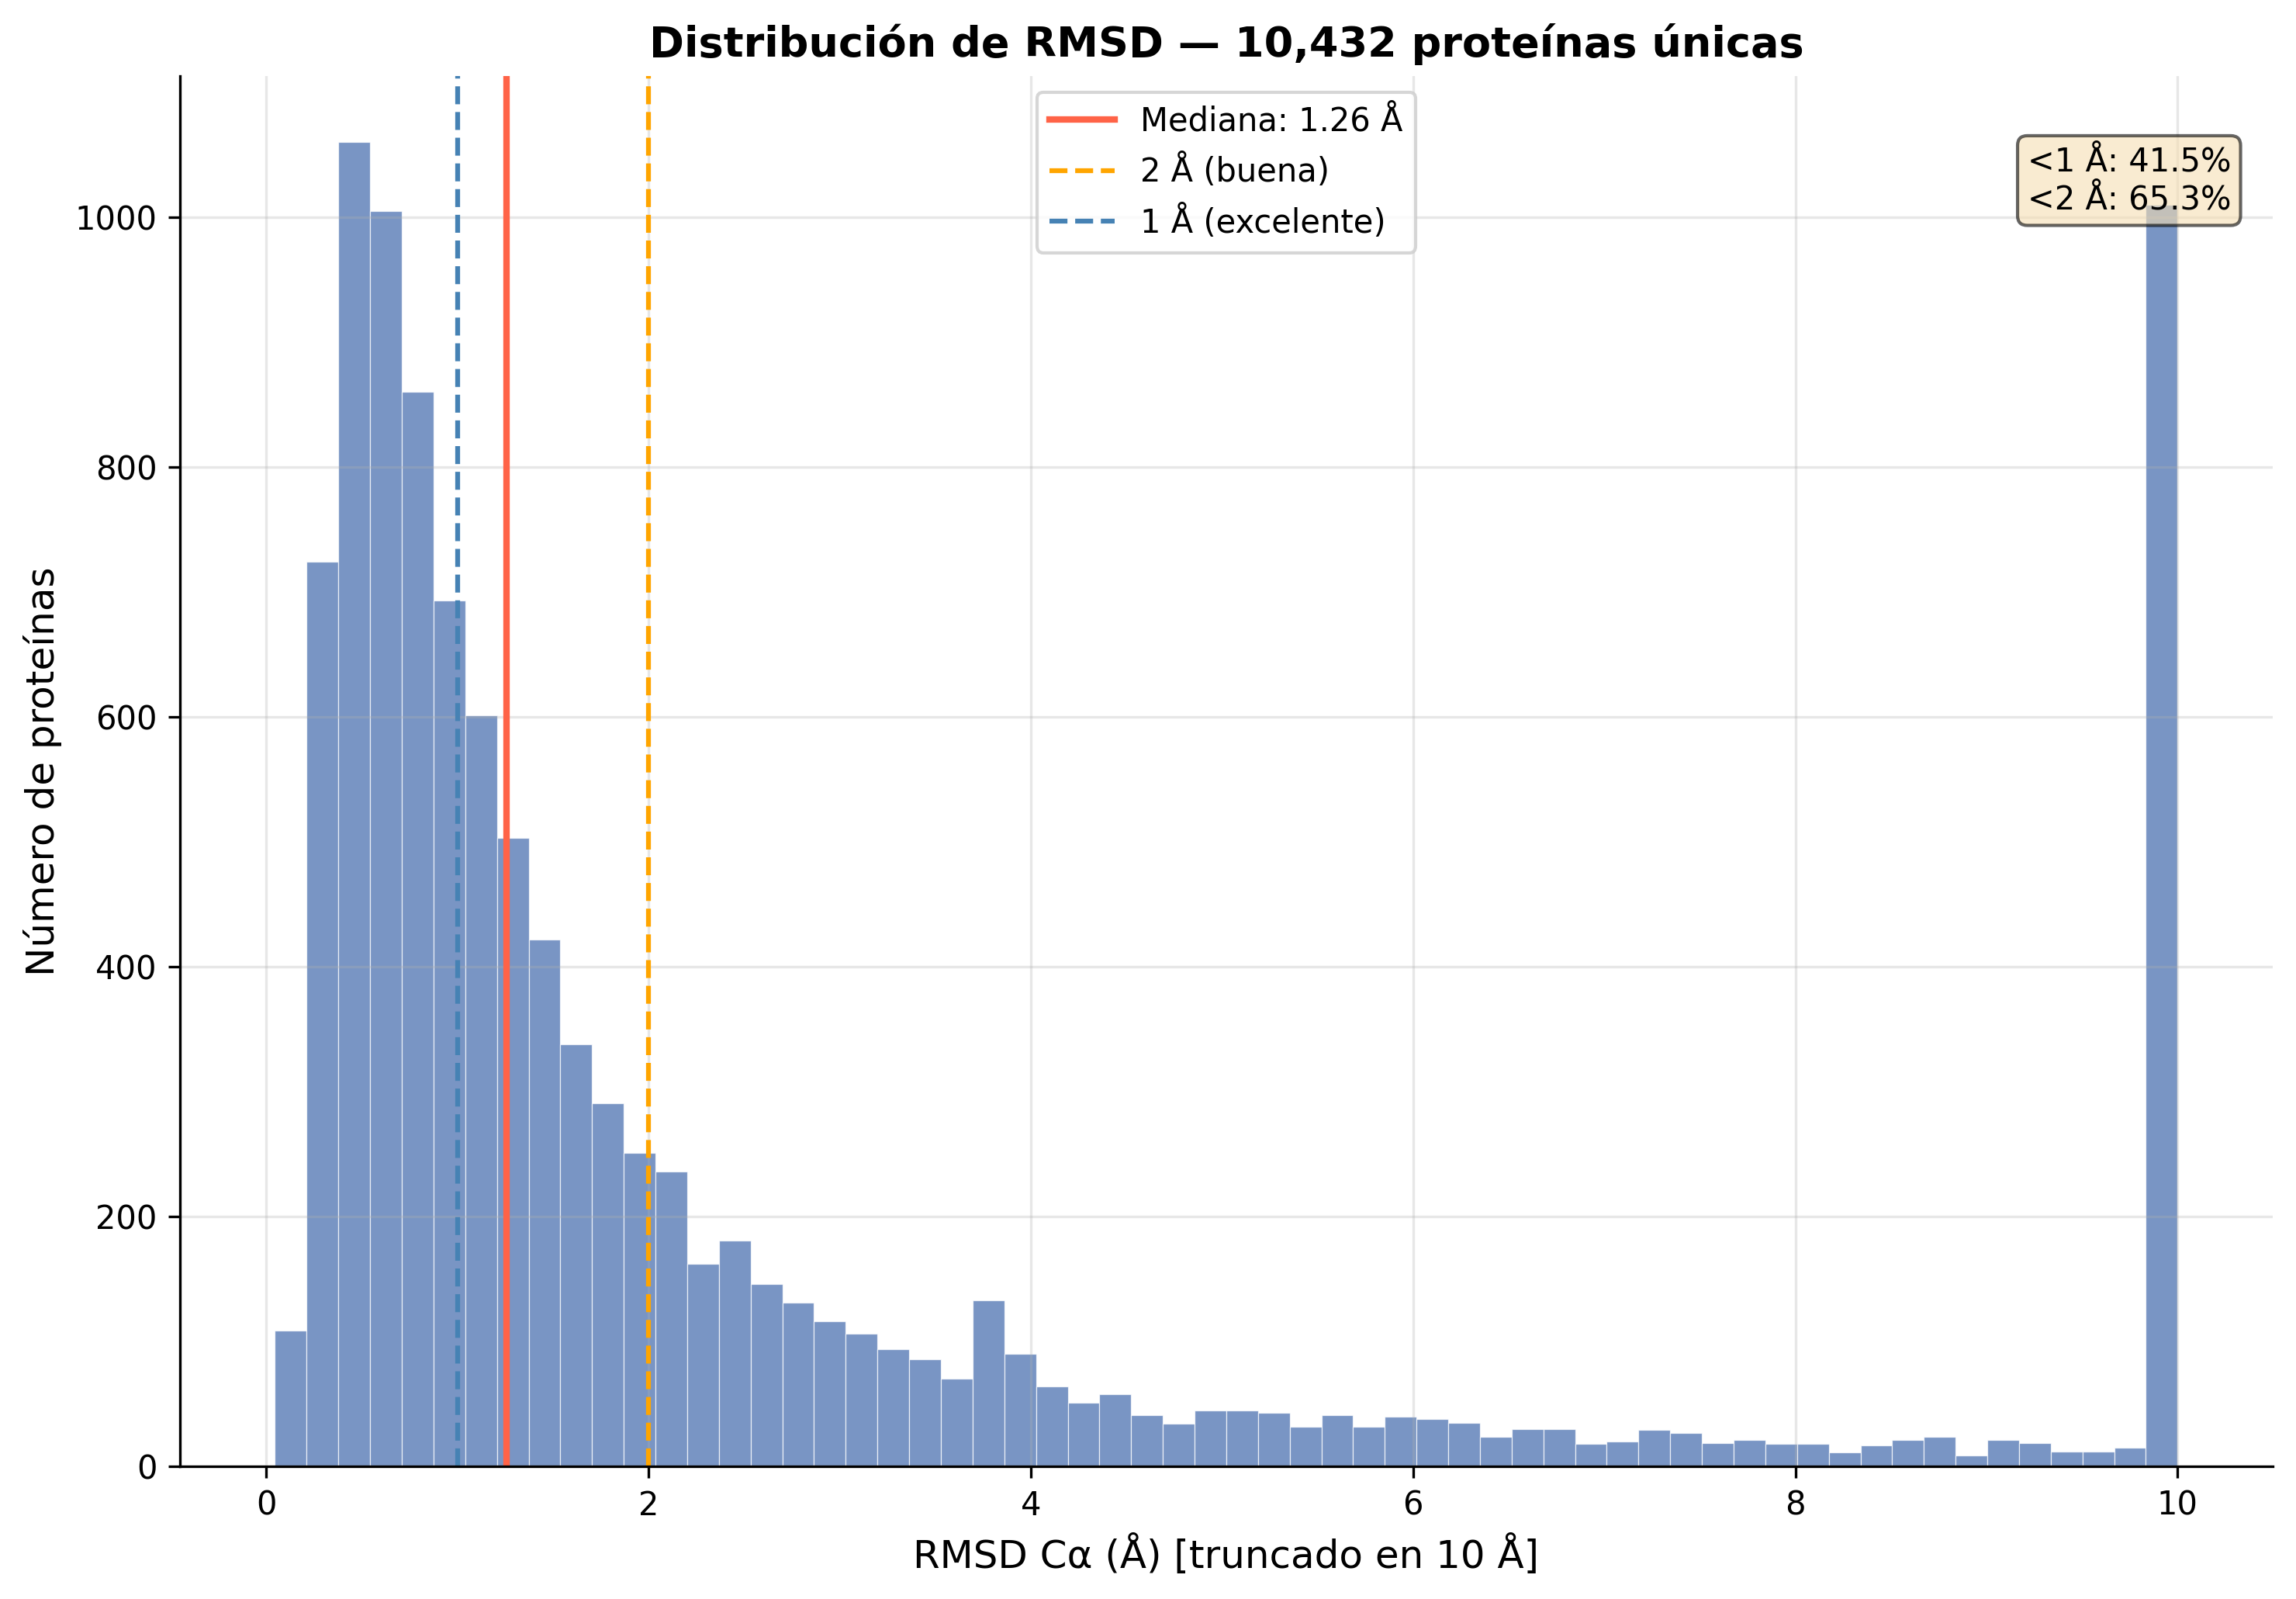
\includegraphics[width=\linewidth]{fig_00c_rmsd_histogram.png}
    \column{0.38\textwidth}
      \begin{block}{Dataset completo}
        \begin{itemize}
          \item 10,432 proteínas únicas
          \item RMSD mediano: 1.26 \AA
          \item RMSD medio: 3.56 \AA
          \item 41.5\% con RMSD $<1$ \AA
          \item 65.3\% con RMSD $<2$ \AA
        \end{itemize}
      \end{block}

      \begin{block}{Lectura}
        La mediana representa mejor el desempeño porque la distribución tiene cola derecha y outliers conformacionales.
      \end{block}
  \end{columns}
\end{frame}

\begin{frame}[t,shrink=8]{Tamaño proteico, impacto y conclusiones}
  \small
  \begin{columns}[T]
    \column{0.54\textwidth}
      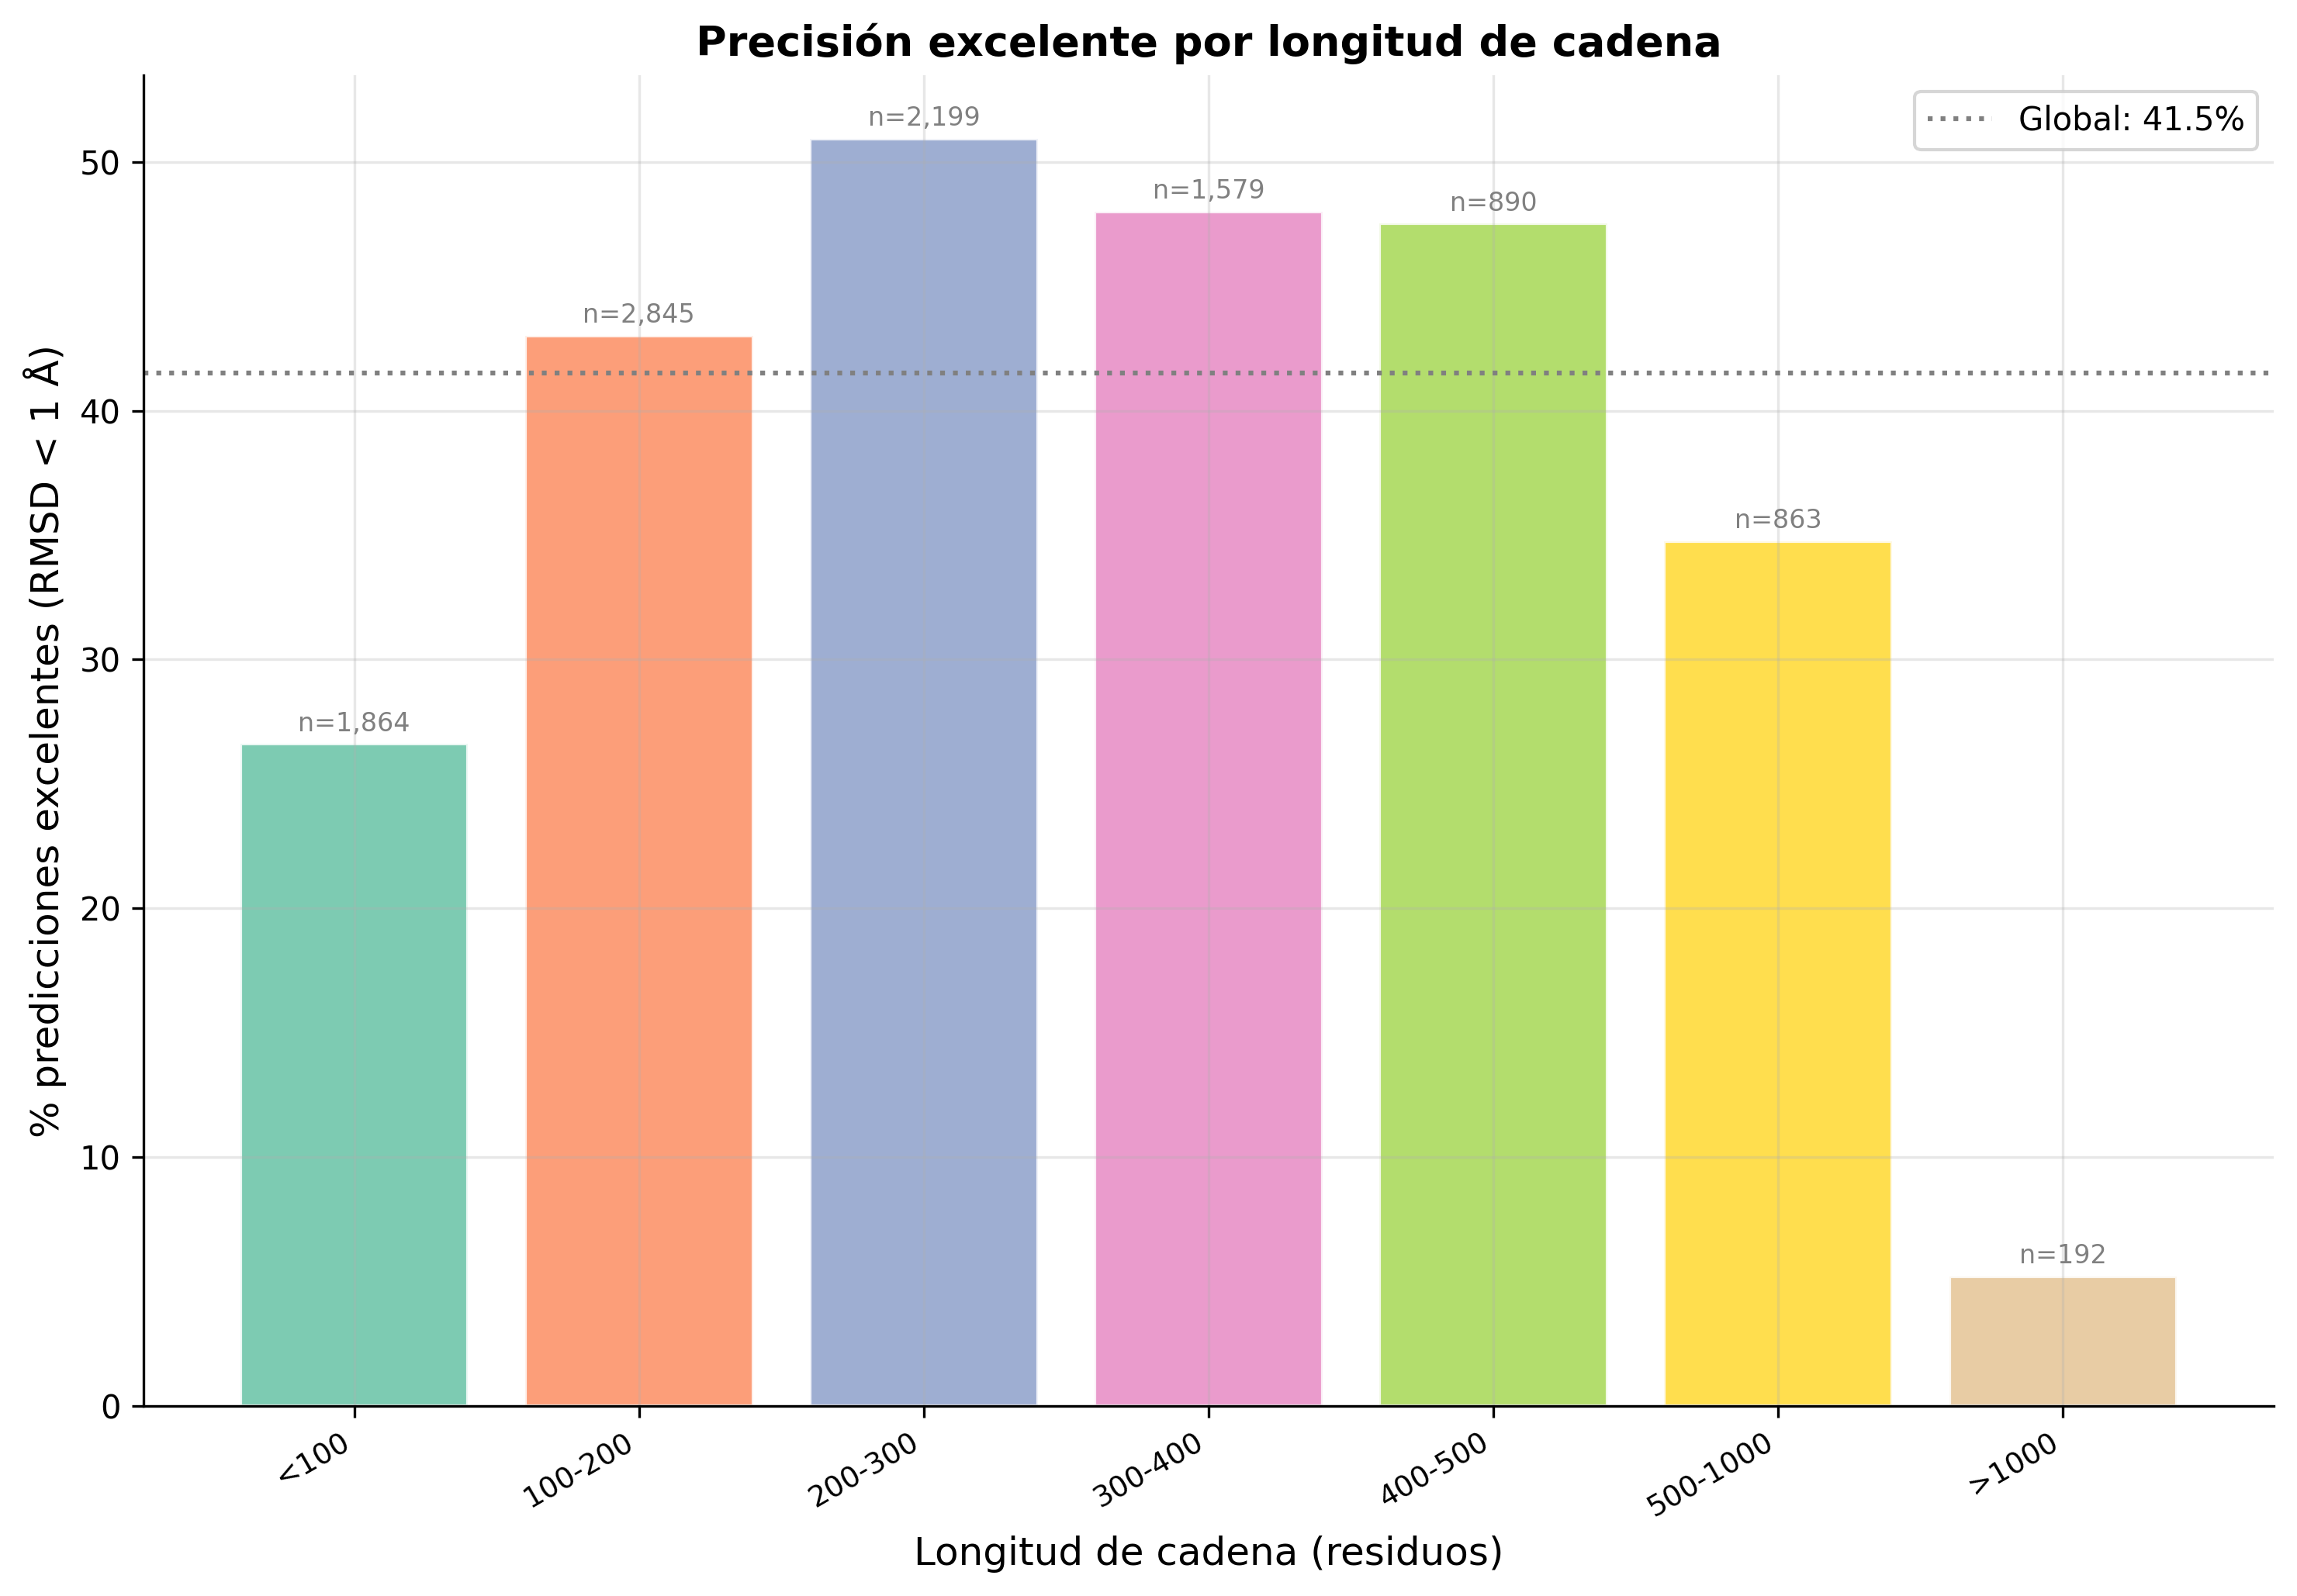
\includegraphics[width=0.96\linewidth]{fig_00d_excellence_by_length.png}
    \column{0.42\textwidth}
      \begin{block}{Tamaño proteico}
        \begin{itemize}
          \item No aparece un sweet spot universal 250--300.
          \item 200--300 residuos: mediana 0.98 \AA.
          \item 300--400 residuos: mediana 1.05 \AA.
          \item $>1000$ residuos: mediana 4.68 \AA.
        \end{itemize}
      \end{block}

      \begin{block}{Conclusiones}
        \begin{itemize}
          \item AlphaFold2 = \textbf{precisión experimental} en 2/3 del proteoma.
          \item SIFTS es \textbf{requisito}; benchmarks sin él son inválidos.
          \item El \emph{sweet spot} 250--300 era artefacto, no biología.
          \item Pipeline transferible a AlphaFold3 y otros predictores.
        \end{itemize}
      \end{block}
  \end{columns}
\end{frame}

\end{document}
